\documentclass{article}

\usepackage[paper=letterpaper,margin=2.5cm]{geometry} % Set Margins

%% Math and math fonts
\usepackage{amsmath, amsthm, amssymb, amsfonts}
\usepackage{amsmath}
\usepackage{bbm} % for \mathbbm{1}

% date
\usepackage[nodayofweek]{datetime}

% Color
\usepackage{color, xcolor}

% Misc
\usepackage{environ}  % \collect@body in asmmath
\usepackage{graphicx} % \includegraphics options
\usepackage{mdframed} % text boxes
\usepackage{indentfirst} % Indent first paragraph after section header
\usepackage[shortlabels]{enumitem} % Control enumerate items with [(a)]
\usepackage{comment} % Comments
\usepackage{fancyhdr} % Headers and footers

% Tables
\usepackage{array}

% Sub-figures and figure placement
\usepackage{caption}
\usepackage{subcaption}
\usepackage{float} 

% Graphing
\usepackage{pgfplots}
\pgfplotsset{compat=1.17}
\usepackage{tikz}

% Title Placement
\usepackage{titling}
\setlength{\droptitle}{-6em}

%set indent to 
\setlength{\parindent}{0pt}

% Hyper refs
\usepackage{hyperref}
\hypersetup{
    colorlinks=true,
    linkcolor=blue,
    urlcolor  = blue,
    filecolor=magenta,      
    urlcolor=blue,
    citecolor = blue,
    anchorcolor = blue
}

% % Citation management
\usepackage{natbib}
\bibliographystyle{abbrvnat}
\setcitestyle{authordate,open={(},close={)}}

\pagestyle{fancy}

\usepackage[paper=letterpaper,margin=2.5cm]{geometry} % Set Margins

%% Math and math fonts
\usepackage{amsmath, amsthm, amssymb, amsfonts}
\usepackage{bbm} % for \mathbbm{1}

% date
\usepackage[nodayofweek]{datetime}

% Color
\usepackage{color, xcolor}

% Misc
\usepackage{environ}  % \collect@body in asmmath
\usepackage{graphicx} % \includegraphics options
\usepackage{mdframed} % text boxes
\usepackage{indentfirst} % Indent first paragraph after section header
\usepackage{comment} % Comments
\usepackage{fancyhdr} % Headers and footers

% Tables
\usepackage{array}

% Sub-figures and figure placement
\usepackage{caption}
% \usepackage{subcaption}
\usepackage{float} 

% Graphing
\usepackage{pgfplots}
\pgfplotsset{compat=1.17}
\usepackage{tikz}

% Title Placement
\usepackage{titling}
\setlength{\droptitle}{-6em}

%set indent to 
\setlength{\parindent}{0pt}

% Hyper refs
\usepackage{hyperref}
\hypersetup{
    colorlinks=true,
    linkcolor=blue,
    urlcolor  = blue,
    filecolor=magenta,      
    urlcolor=blue,
    citecolor = blue,
    anchorcolor = blue
}

% % Citation management
\usepackage{natbib}
\bibliographystyle{abbrvnat}
\setcitestyle{authordate,open={(},close={)}}

% ----------------------------------------
% TITLE
% ----------------------------------------

\pagestyle{fancy}

\lhead{Creel}
\chead{Probability and Integrals}
\rhead{AMES}

\title{AMES Class Notes -- Week 7, Wednesday: Probability}
\author{Andie Creel}

\begin{document}
\maketitle

\section{Random Variables and probability density functions}

A \textbf{random variable} \( Y \) is not inherently random, and while it's called a "variable," it behaves more like a \textit{function} that maps outcomes from a sample space to real numbers (or another set of values). The randomness comes from the fact that the outcome it maps to depends on the result of some random process.\\

\textbf{Key Clarifications:}

\begin{itemize}
    \item \textbf{Random Variable \( Y \)}: This is a function that assigns a number to each possible outcome of a random experiment. It describes a \textbf{distribution} over possible values, i.e., the probabilities of different outcomes. The distribution of \( Y \) gives us the likelihood of each possible value that \( Y \) can take.

    \item \textbf{Specific Value \( y \)}: When we observe or "draw" a specific value from this distribution, we denote it as lowercase \( y \). This is a specific realization or outcome of the random variable \( Y \). For example, if \( Y \) represents the distribution of grades, then \( y \) might represent a specific grade, such as 90\%.
\end{itemize}

\textbf{Example:}
\begin{itemize}
    \item \( Y \): Represents a random variable describing people's grades, and this random variable is associated with a \textbf{distribution} of grades (e.g., a normal distribution of grades in a class).
    \item \( y \): Represents a specific value that the random variable \( Y \) can take, such as a grade of 90\%.
\end{itemize}

Thus, \( Y \) describes the entire distribution, and \( y \) is one particular outcome from that distribution.


\section{Normal Distribution}
If the random variable $Y$ is distributed normally it will look like 
\begin{align}
    Y = f(y) = \int_{- \infty}^{\infty} \frac{1}{\sigma \sqrt{2 \pi}} e^{-\frac{1}{2}(\frac{y - \mu}{\sigma})^2} dy = 1
\end{align}

the inside of the integral is the probability density function. The integral of a pdf must equal 1. 

\subsection{Defining probability density function (integral of pdf will equal 1)}
Consider the random variable $Y$ that has the probability density function (pdf), $f(y)$
\begin{align}
    Y = f(y) = 2y e^{-y^2} \label{pdf}
\end{align}

and the support is $[0, \infty )$. Definitionally, the area under the pdf will equal 1, because the pdf describes the probability of a random draw of $Y$ equalling $y$. Because a draw of $Y$ needs to equal something, when you sum up the probabilities of it equally all possible values that needs to sum to 1 (100\% chance it does equal something).  \\

Our cumulative distribution function (CDF) is 
\begin{align}
    CDF &= \int_0^\infty 2y e^{-y^2} dy \\
    &= 2 \int_0^\infty y e^{-y^2} dy
\end{align}

Let $u = -y^2$, $du = -2y dy$
\begin{align}
    &= 2 \int_0^\infty  ye^u \frac{du}{-2y} \\
    &= -1  \int_0^\infty e^u du \\
    &= -1 e^u \bigg |_0^\infty \\
    & = -1 e^{-y^2}\bigg |_0^\infty \label{pdf_int}\\ 
    & = 0 - - 1\\
    & = 1
\end{align}

Which integrates to 1 after doing a u substitution, and so we know we have a proper pdf. \textbf{The integral of a pdf will definitionally be one.}\\

\section{Finding median of a random variable using pdf}
What if you want to find the \textbf{median}? Set the CDF equal to $0.5$ because the median is the 50th percentile. \\

The unknown is the point on the x-axis (Fig 1) where the area under the pdf is equal to 0.5 (which is defined as our median). Start with equation \ref{pdf_int} from our previous integral derivation because we know the integral is equal to that. But replace the upper bound to an unknown $\tilde{y}$ which will be the $y$ value where "half the pdf is the the left" of it and "half is to the right", aka it's our median and we set the CDF from 0 to $\tilde y$ equal to 0.5.

\begin{align}
    -1 e^{-y^2} \bigg |_0^{\tilde {y}} &= 0.5\\
    -e^{- \tilde y ^2} - - 1 &= 0. 5\\
    -e^{- \tilde y ^2} &= - 0.5 \\  
    e^{- \tilde y ^2} & = 0.5\\
    ln( e^{- \tilde y ^2}) &= ln(1/2) \\
    - \tilde y^2 &= ln(1/2)  \\
    \tilde y^2 &= - ln(1/2) \\
    \tilde y &= \sqrt{-ln(1/2)}
\end{align}

so we know that the median value of the random variable $Y$ with the pdf in equation \ref{pdf} is $ \tilde y = \sqrt{- ln(1/2)}$.

\begin{figure}[htp]
    \centering
        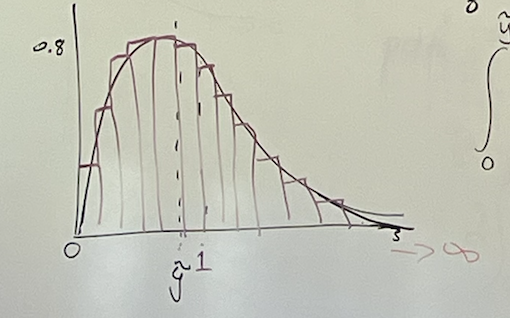
\includegraphics[width=0.5\textwidth]{Screen Shot 2023-10-09 at 11.11.30 AM.png}
    \caption{Histograph}
    % \label{fig:sample}
\end{figure}

\section{Finding the mean of a random variable using the pdf}
To find a mean, we sum the values and divide it by the number of people we summed over. This is the same as multiplying everyone's value by $\frac{1}{N}$, 
\begin{align}
   E[Y]= \bar y &= \frac{1}{N}\sum_n y_n\\
   &= \sum_n \frac{1}{N} y_n
\end{align}
where the \textbf{expectation function} $E[Y]$ is the same as saying the mean. \\

We can use the pdf to get our mean! The pdf would replace the $\frac{1}{N}$ and the sum would be replaced by the integral. 

\begin{align}
    E[Y]= \bar y = \int_0^\infty 2ye^{-y^2} * y dy
\end{align}

Where the integral sign replaces the summation, and the pdf from equation \ref{pdf} replaces $1/N$. This is similar to how you may have taken weighted means in the past. \\

The general rule for finding the mean of a random variable by using the pdf $f(y)$ of that random variable is 
\begin{align}
    E[Y] = \int_\Omega y f(y) dy
\end{align}
where $\Omega$ is the support of $y$ (aka any values that the random variable $Y$ can equal). \\


\section{Uniform Distribution Example}
Consider the uniform distribution's pdf 
\begin{align}
    f(y) = \frac{1}{\theta_2 - \theta_1} \label{unif_pdf}
\end{align}
Let $\theta_2 = 1$ and $\theta_1 = 0$, which is the same as saying that the random variable $Y$ is only supported over $y$ values of 0 to 1. 

\begin{align}
    f(y) = \frac{1}{1 - 0}\\
    f(y) = 1
\end{align}

Prove $f(y)$ \textbf{is a pdf} by showing it integrates to 1. 
\begin{align}
    \int_0^1 1 dy = y \bigg|_0^1 = 1 - 0 = 1
\end{align}

What's the mean? 
\begin{align}
    E(Y) = \int_0^1 y *1 dy = \frac{1}{2} y^2 \bigg|_0^1 = \frac{1}{2}
\end{align}

What's the median? 
\begin{align}
    Med(Y) = \int_0^{\tilde y} dy = 0.5 \\
    y\bigg|_0^{\tilde y} = 0.5 \\
    \tilde y - 0 = 0.5
\end{align}




\section{Finding the variance of a random variable using the pdf}

We can find the variance of a random variable $Y$ by considering the squared deviations of a variable $y$ from the mean $ E[Y] = \mu$. Our equation for variance is 
\begin{align}
    VAR(Y) = E(Y^2) -[E(Y)]^2 
\end{align}

We an use the pdf to find the variance of $Y$, as well, because we can use the pdf to find a mean,
\begin{align}
        VAR(Y) = \int_\Omega y^2 f(y) dy - E(Y)^2 \label{var}
\end{align}


\subsection{What's the variance of random variable $Y$ with a uniform distribution?}
Let's use \ref{var} to find the variance. We already known $E(Y) = 1/2$ from the section above. But how do we get $E(Y^2)$?\\

We can use the pdf to find the expectation of a \textit{function} of the random variable, which is what $E(Y^2)$ is. \\

\textbf{Finding the mean of a \textit{function} of a random variable using the pdf}

Let's say you're  interested in $g(y)$ rather that $y$ itself.
\begin{align}
    E[g(y)] = \int_\Omega g(y) f(y) dy
\end{align}
where $f(y)$ continues to be the pdf of $Y$. This doesn't break jensen's inequality. \\

In our current case, $g(Y) = Y^2$\\ 
 
Nowe we can retun to finding the variance. Recall the uniform pdf from equation \ref{unif_pdf} and that we're assuming the support of random variable $Y$ is 0 to 1, and the $E[Y]$ of the uniformly distributed variable is 1/2.

\begin{align}
    Var(Y) &= \int_0^1 y^2 dy - \frac{1}{2}^2\\
    &= \frac{1}{3}y^3 \bigg|_0^1  -  \frac{1}{2}^2  \\
    &= \frac{1}{3} - \frac{1}{4} \\
    &= \frac{1}{12}
\end{align}

\end{document}